\begin{frame}{Cost function}
    \begin{columns}
      \column{0.33\textwidth}
      \centering
      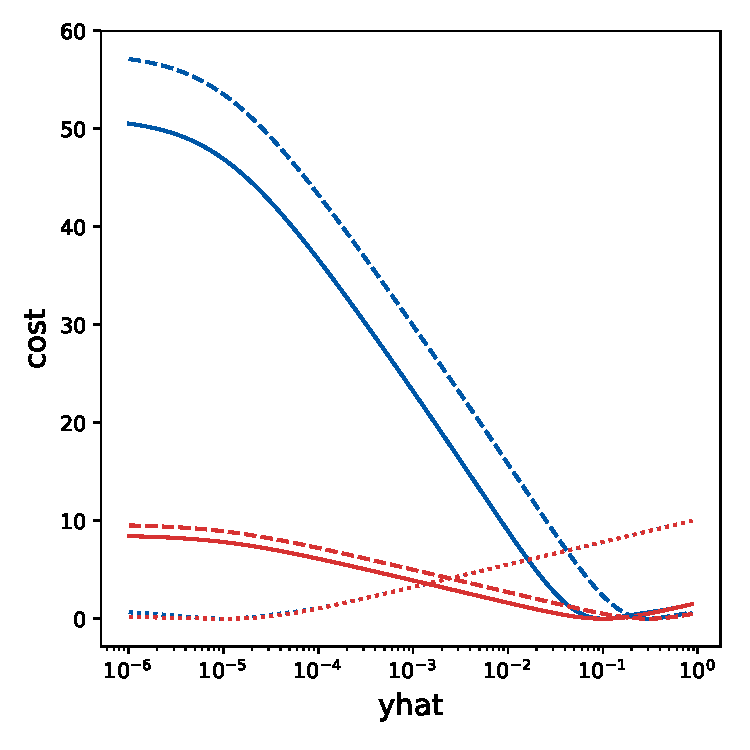
\includegraphics[width=\textwidth, trim=20 0 20 0]{images/Asym_CostPlot_190302.pdf}
      \column{0.33\textwidth}
      \centering
      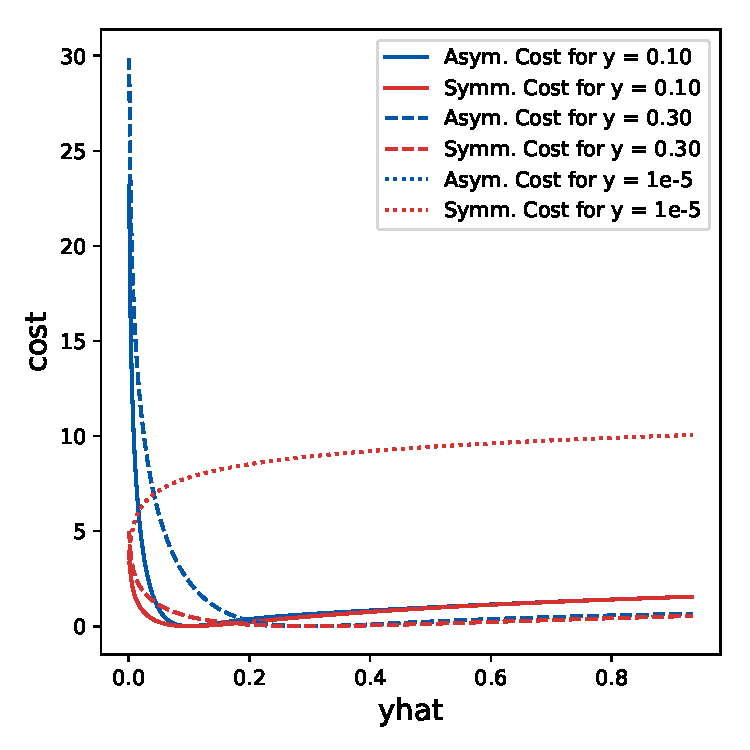
\includegraphics[width=\textwidth, trim=20 0 20 0]{images/Asym_CostPlot_190302_linear.pdf}
      \column{0.33\textwidth}
      \centering
      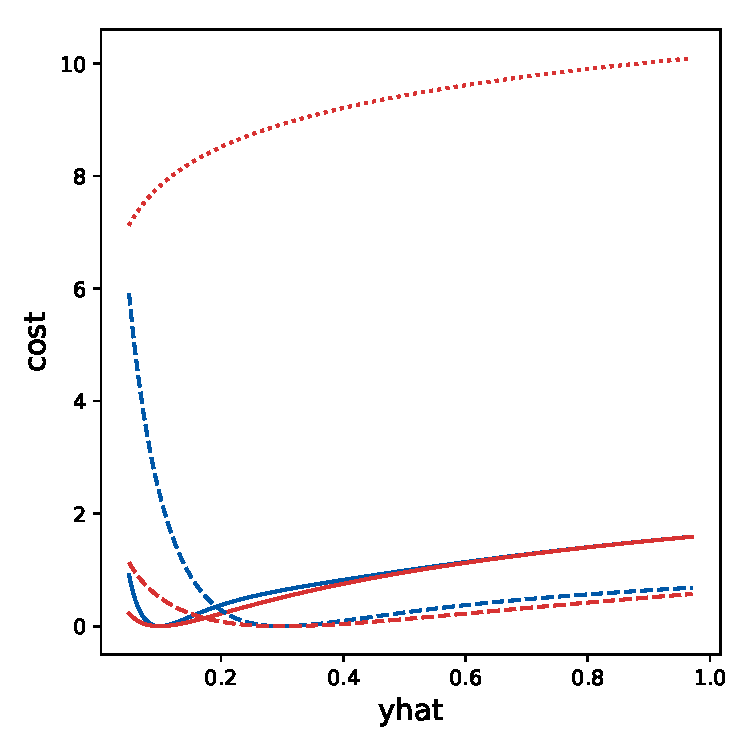
\includegraphics[width=\textwidth, trim=20 0 20 0]{images/Asym_CostPlot_190302_linearA.pdf}
      \end{columns}


    \begin{block}{Approach}
      \begin{itemize}
         \item Symmetric cost function: low FP but low efficiency
         \item Adding asymmetry term controls trade-off for FP vs.\ efficiency
     \end{itemize}
    \end{block}
\end{frame}
